% Options for packages loaded elsewhere
% Options for packages loaded elsewhere
\PassOptionsToPackage{unicode}{hyperref}
\PassOptionsToPackage{hyphens}{url}
\PassOptionsToPackage{dvipsnames,svgnames,x11names}{xcolor}
%
\documentclass[
  letterpaper,
  DIV=11,
  numbers=noendperiod]{scrartcl}
\usepackage{xcolor}
\usepackage{amsmath,amssymb}
\setcounter{secnumdepth}{-\maxdimen} % remove section numbering
\usepackage{iftex}
\ifPDFTeX
  \usepackage[T1]{fontenc}
  \usepackage[utf8]{inputenc}
  \usepackage{textcomp} % provide euro and other symbols
\else % if luatex or xetex
  \usepackage{unicode-math} % this also loads fontspec
  \defaultfontfeatures{Scale=MatchLowercase}
  \defaultfontfeatures[\rmfamily]{Ligatures=TeX,Scale=1}
\fi
\usepackage{lmodern}
\ifPDFTeX\else
  % xetex/luatex font selection
\fi
% Use upquote if available, for straight quotes in verbatim environments
\IfFileExists{upquote.sty}{\usepackage{upquote}}{}
\IfFileExists{microtype.sty}{% use microtype if available
  \usepackage[]{microtype}
  \UseMicrotypeSet[protrusion]{basicmath} % disable protrusion for tt fonts
}{}
\makeatletter
\@ifundefined{KOMAClassName}{% if non-KOMA class
  \IfFileExists{parskip.sty}{%
    \usepackage{parskip}
  }{% else
    \setlength{\parindent}{0pt}
    \setlength{\parskip}{6pt plus 2pt minus 1pt}}
}{% if KOMA class
  \KOMAoptions{parskip=half}}
\makeatother
% Make \paragraph and \subparagraph free-standing
\makeatletter
\ifx\paragraph\undefined\else
  \let\oldparagraph\paragraph
  \renewcommand{\paragraph}{
    \@ifstar
      \xxxParagraphStar
      \xxxParagraphNoStar
  }
  \newcommand{\xxxParagraphStar}[1]{\oldparagraph*{#1}\mbox{}}
  \newcommand{\xxxParagraphNoStar}[1]{\oldparagraph{#1}\mbox{}}
\fi
\ifx\subparagraph\undefined\else
  \let\oldsubparagraph\subparagraph
  \renewcommand{\subparagraph}{
    \@ifstar
      \xxxSubParagraphStar
      \xxxSubParagraphNoStar
  }
  \newcommand{\xxxSubParagraphStar}[1]{\oldsubparagraph*{#1}\mbox{}}
  \newcommand{\xxxSubParagraphNoStar}[1]{\oldsubparagraph{#1}\mbox{}}
\fi
\makeatother

\usepackage{color}
\usepackage{fancyvrb}
\newcommand{\VerbBar}{|}
\newcommand{\VERB}{\Verb[commandchars=\\\{\}]}
\DefineVerbatimEnvironment{Highlighting}{Verbatim}{commandchars=\\\{\}}
% Add ',fontsize=\small' for more characters per line
\usepackage{framed}
\definecolor{shadecolor}{RGB}{241,243,245}
\newenvironment{Shaded}{\begin{snugshade}}{\end{snugshade}}
\newcommand{\AlertTok}[1]{\textcolor[rgb]{0.68,0.00,0.00}{#1}}
\newcommand{\AnnotationTok}[1]{\textcolor[rgb]{0.37,0.37,0.37}{#1}}
\newcommand{\AttributeTok}[1]{\textcolor[rgb]{0.40,0.45,0.13}{#1}}
\newcommand{\BaseNTok}[1]{\textcolor[rgb]{0.68,0.00,0.00}{#1}}
\newcommand{\BuiltInTok}[1]{\textcolor[rgb]{0.00,0.23,0.31}{#1}}
\newcommand{\CharTok}[1]{\textcolor[rgb]{0.13,0.47,0.30}{#1}}
\newcommand{\CommentTok}[1]{\textcolor[rgb]{0.37,0.37,0.37}{#1}}
\newcommand{\CommentVarTok}[1]{\textcolor[rgb]{0.37,0.37,0.37}{\textit{#1}}}
\newcommand{\ConstantTok}[1]{\textcolor[rgb]{0.56,0.35,0.01}{#1}}
\newcommand{\ControlFlowTok}[1]{\textcolor[rgb]{0.00,0.23,0.31}{\textbf{#1}}}
\newcommand{\DataTypeTok}[1]{\textcolor[rgb]{0.68,0.00,0.00}{#1}}
\newcommand{\DecValTok}[1]{\textcolor[rgb]{0.68,0.00,0.00}{#1}}
\newcommand{\DocumentationTok}[1]{\textcolor[rgb]{0.37,0.37,0.37}{\textit{#1}}}
\newcommand{\ErrorTok}[1]{\textcolor[rgb]{0.68,0.00,0.00}{#1}}
\newcommand{\ExtensionTok}[1]{\textcolor[rgb]{0.00,0.23,0.31}{#1}}
\newcommand{\FloatTok}[1]{\textcolor[rgb]{0.68,0.00,0.00}{#1}}
\newcommand{\FunctionTok}[1]{\textcolor[rgb]{0.28,0.35,0.67}{#1}}
\newcommand{\ImportTok}[1]{\textcolor[rgb]{0.00,0.46,0.62}{#1}}
\newcommand{\InformationTok}[1]{\textcolor[rgb]{0.37,0.37,0.37}{#1}}
\newcommand{\KeywordTok}[1]{\textcolor[rgb]{0.00,0.23,0.31}{\textbf{#1}}}
\newcommand{\NormalTok}[1]{\textcolor[rgb]{0.00,0.23,0.31}{#1}}
\newcommand{\OperatorTok}[1]{\textcolor[rgb]{0.37,0.37,0.37}{#1}}
\newcommand{\OtherTok}[1]{\textcolor[rgb]{0.00,0.23,0.31}{#1}}
\newcommand{\PreprocessorTok}[1]{\textcolor[rgb]{0.68,0.00,0.00}{#1}}
\newcommand{\RegionMarkerTok}[1]{\textcolor[rgb]{0.00,0.23,0.31}{#1}}
\newcommand{\SpecialCharTok}[1]{\textcolor[rgb]{0.37,0.37,0.37}{#1}}
\newcommand{\SpecialStringTok}[1]{\textcolor[rgb]{0.13,0.47,0.30}{#1}}
\newcommand{\StringTok}[1]{\textcolor[rgb]{0.13,0.47,0.30}{#1}}
\newcommand{\VariableTok}[1]{\textcolor[rgb]{0.07,0.07,0.07}{#1}}
\newcommand{\VerbatimStringTok}[1]{\textcolor[rgb]{0.13,0.47,0.30}{#1}}
\newcommand{\WarningTok}[1]{\textcolor[rgb]{0.37,0.37,0.37}{\textit{#1}}}

\usepackage{longtable,booktabs,array}
\usepackage{calc} % for calculating minipage widths
% Correct order of tables after \paragraph or \subparagraph
\usepackage{etoolbox}
\makeatletter
\patchcmd\longtable{\par}{\if@noskipsec\mbox{}\fi\par}{}{}
\makeatother
% Allow footnotes in longtable head/foot
\IfFileExists{footnotehyper.sty}{\usepackage{footnotehyper}}{\usepackage{footnote}}
\makesavenoteenv{longtable}
\usepackage{graphicx}
\makeatletter
\newsavebox\pandoc@box
\newcommand*\pandocbounded[1]{% scales image to fit in text height/width
  \sbox\pandoc@box{#1}%
  \Gscale@div\@tempa{\textheight}{\dimexpr\ht\pandoc@box+\dp\pandoc@box\relax}%
  \Gscale@div\@tempb{\linewidth}{\wd\pandoc@box}%
  \ifdim\@tempb\p@<\@tempa\p@\let\@tempa\@tempb\fi% select the smaller of both
  \ifdim\@tempa\p@<\p@\scalebox{\@tempa}{\usebox\pandoc@box}%
  \else\usebox{\pandoc@box}%
  \fi%
}
% Set default figure placement to htbp
\def\fps@figure{htbp}
\makeatother


% definitions for citeproc citations
\NewDocumentCommand\citeproctext{}{}
\NewDocumentCommand\citeproc{mm}{%
  \begingroup\def\citeproctext{#2}\cite{#1}\endgroup}
\makeatletter
 % allow citations to break across lines
 \let\@cite@ofmt\@firstofone
 % avoid brackets around text for \cite:
 \def\@biblabel#1{}
 \def\@cite#1#2{{#1\if@tempswa , #2\fi}}
\makeatother
\newlength{\cslhangindent}
\setlength{\cslhangindent}{1.5em}
\newlength{\csllabelwidth}
\setlength{\csllabelwidth}{3em}
\newenvironment{CSLReferences}[2] % #1 hanging-indent, #2 entry-spacing
 {\begin{list}{}{%
  \setlength{\itemindent}{0pt}
  \setlength{\leftmargin}{0pt}
  \setlength{\parsep}{0pt}
  % turn on hanging indent if param 1 is 1
  \ifodd #1
   \setlength{\leftmargin}{\cslhangindent}
   \setlength{\itemindent}{-1\cslhangindent}
  \fi
  % set entry spacing
  \setlength{\itemsep}{#2\baselineskip}}}
 {\end{list}}
\usepackage{calc}
\newcommand{\CSLBlock}[1]{\hfill\break\parbox[t]{\linewidth}{\strut\ignorespaces#1\strut}}
\newcommand{\CSLLeftMargin}[1]{\parbox[t]{\csllabelwidth}{\strut#1\strut}}
\newcommand{\CSLRightInline}[1]{\parbox[t]{\linewidth - \csllabelwidth}{\strut#1\strut}}
\newcommand{\CSLIndent}[1]{\hspace{\cslhangindent}#1}



\setlength{\emergencystretch}{3em} % prevent overfull lines

\providecommand{\tightlist}{%
  \setlength{\itemsep}{0pt}\setlength{\parskip}{0pt}}



 


\KOMAoption{captions}{tableheading}
\makeatletter
\@ifpackageloaded{caption}{}{\usepackage{caption}}
\AtBeginDocument{%
\ifdefined\contentsname
  \renewcommand*\contentsname{Table of contents}
\else
  \newcommand\contentsname{Table of contents}
\fi
\ifdefined\listfigurename
  \renewcommand*\listfigurename{List of Figures}
\else
  \newcommand\listfigurename{List of Figures}
\fi
\ifdefined\listtablename
  \renewcommand*\listtablename{List of Tables}
\else
  \newcommand\listtablename{List of Tables}
\fi
\ifdefined\figurename
  \renewcommand*\figurename{Figure}
\else
  \newcommand\figurename{Figure}
\fi
\ifdefined\tablename
  \renewcommand*\tablename{Table}
\else
  \newcommand\tablename{Table}
\fi
}
\@ifpackageloaded{float}{}{\usepackage{float}}
\floatstyle{ruled}
\@ifundefined{c@chapter}{\newfloat{codelisting}{h}{lop}}{\newfloat{codelisting}{h}{lop}[chapter]}
\floatname{codelisting}{Listing}
\newcommand*\listoflistings{\listof{codelisting}{List of Listings}}
\makeatother
\makeatletter
\makeatother
\makeatletter
\@ifpackageloaded{caption}{}{\usepackage{caption}}
\@ifpackageloaded{subcaption}{}{\usepackage{subcaption}}
\makeatother
\usepackage{bookmark}
\IfFileExists{xurl.sty}{\usepackage{xurl}}{} % add URL line breaks if available
\urlstyle{same}
\hypersetup{
  pdftitle={Thesis Defense},
  pdfauthor={Robin P. van de Water},
  colorlinks=true,
  linkcolor={blue},
  filecolor={Maroon},
  citecolor={Blue},
  urlcolor={Blue},
  pdfcreator={LaTeX via pandoc}}


\title{Thesis Defense}
\usepackage{etoolbox}
\makeatletter
\providecommand{\subtitle}[1]{% add subtitle to \maketitle
  \apptocmd{\@title}{\par {\large #1 \par}}{}{}
}
\makeatother
\subtitle{Thesis Defense Robin P. van de Water}
\author{}
\date{}
\begin{document}
\maketitle


\subsection{Hello, There}\label{hello-there}

This presentation will show you examples of what you can do with Quarto
and \href{https://revealjs.com}{Reveal.js}, including

\begin{itemize}
\tightlist
\item
  Presenting code and LaTeX equations (Schadow et al. 1999)
\item
  Including computations in slide output render (Chishtie et al. 2023)
\item
  Image, video, and iframe backgrounds
\item
  Fancy transitions and animations
\item
  Activating scroll view.
\end{itemize}

\ldots and much more

\subsection{Pretty Code}\label{pretty-code}

\begin{itemize}
\tightlist
\item
  Over 20 syntax highlighting themes available
\item
  Default theme optimized for accessibility
\end{itemize}

\begin{Shaded}
\begin{Highlighting}[]
\CommentTok{\# Define a server for the Shiny app}
\ControlFlowTok{function}\NormalTok{(input, output) \{}
  
  \CommentTok{\# Fill in the spot we created for a plot}
\NormalTok{  output}\SpecialCharTok{$}\NormalTok{phonePlot }\OtherTok{\textless{}{-}} \FunctionTok{renderPlot}\NormalTok{(\{}
    \CommentTok{\# Render a barplot}
\NormalTok{  \})}
\NormalTok{\}}
\end{Highlighting}
\end{Shaded}

Learn more:
\href{https://?meta:prerelease-subdomainquarto.org/docs/output-formats/html-code.html\#highlighting}{Syntax
Highlighting}

\subsection{Code Animations}\label{code-animations}

\begin{itemize}
\tightlist
\item
  Over 20 syntax highlighting themes available
\item
  Default theme optimized for accessibility
\end{itemize}

\begin{Shaded}
\begin{Highlighting}[]
\CommentTok{\# Define a server for the Shiny app}
\ControlFlowTok{function}\NormalTok{(input, output) \{}
  
  \CommentTok{\# Fill in the spot we created for a plot}
\NormalTok{  output}\SpecialCharTok{$}\NormalTok{phonePlot }\OtherTok{\textless{}{-}} \FunctionTok{renderPlot}\NormalTok{(\{}
    \CommentTok{\# Render a barplot}
    \FunctionTok{barplot}\NormalTok{(WorldPhones[,input}\SpecialCharTok{$}\NormalTok{region]}\SpecialCharTok{*}\DecValTok{1000}\NormalTok{, }
            \AttributeTok{main=}\NormalTok{input}\SpecialCharTok{$}\NormalTok{region,}
            \AttributeTok{ylab=}\StringTok{"Number of Telephones"}\NormalTok{,}
            \AttributeTok{xlab=}\StringTok{"Year"}\NormalTok{)}
\NormalTok{  \})}
\NormalTok{\}}
\end{Highlighting}
\end{Shaded}

Learn more:
\href{https://?meta:prerelease-subdomainquarto.org/docs/presentations/revealjs/advanced.html\#code-animations}{Code
Animations}

\subsection{Line Highlighting}\label{line-highlighting}

\begin{itemize}
\tightlist
\item
  Highlight specific lines for emphasis
\item
  Incrementally highlight additional lines
\end{itemize}

\begin{Shaded}
\begin{Highlighting}[numbers=left,,]
\ImportTok{import}\NormalTok{ numpy }\ImportTok{as}\NormalTok{ np}
\ImportTok{import}\NormalTok{ matplotlib.pyplot }\ImportTok{as}\NormalTok{ plt}

\NormalTok{r }\OperatorTok{=}\NormalTok{ np.arange(}\DecValTok{0}\NormalTok{, }\DecValTok{2}\NormalTok{, }\FloatTok{0.01}\NormalTok{)}
\NormalTok{theta }\OperatorTok{=} \DecValTok{2} \OperatorTok{*}\NormalTok{ np.pi }\OperatorTok{*}\NormalTok{ r}
\NormalTok{fig, ax }\OperatorTok{=}\NormalTok{ plt.subplots(subplot\_kw}\OperatorTok{=}\NormalTok{\{}\StringTok{\textquotesingle{}projection\textquotesingle{}}\NormalTok{: }\StringTok{\textquotesingle{}polar\textquotesingle{}}\NormalTok{\})}
\NormalTok{ax.plot(theta, r)}
\NormalTok{ax.set\_rticks([}\FloatTok{0.5}\NormalTok{, }\DecValTok{1}\NormalTok{, }\FloatTok{1.5}\NormalTok{, }\DecValTok{2}\NormalTok{])}
\NormalTok{ax.grid(}\VariableTok{True}\NormalTok{)}
\NormalTok{plt.show()}
\end{Highlighting}
\end{Shaded}

Learn more:
\href{https://?meta:prerelease-subdomainquarto.org/docs/presentations/revealjs/\#line-highlighting}{Line
Highlighting}

\subsection{Executable Code}\label{executable-code}

\begin{Shaded}
\begin{Highlighting}[]
\FunctionTok{library}\NormalTok{(ggplot2)}
\FunctionTok{ggplot}\NormalTok{(mtcars, }\FunctionTok{aes}\NormalTok{(hp, mpg, }\AttributeTok{color =}\NormalTok{ am)) }\SpecialCharTok{+}
  \FunctionTok{geom\_point}\NormalTok{() }\SpecialCharTok{+}
  \FunctionTok{geom\_smooth}\NormalTok{(}\AttributeTok{formula =}\NormalTok{ y }\SpecialCharTok{\textasciitilde{}}\NormalTok{ x, }\AttributeTok{method =} \StringTok{"loess"}\NormalTok{)}
\end{Highlighting}
\end{Shaded}

\begin{verbatim}
Warning: The following aesthetics were dropped during statistical transformation:
colour.
i This can happen when ggplot fails to infer the correct grouping structure in
  the data.
i Did you forget to specify a `group` aesthetic or to convert a numerical
  variable into a factor?
\end{verbatim}

\pandocbounded{\includegraphics[keepaspectratio]{index_files/figure-pdf/unnamed-chunk-1-1.pdf}}

Learn more:
\href{https://?meta:prerelease-subdomainquarto.org/docs/presentations/revealjs/\#executable-code}{Executable
Code}

\subsection{LaTeX Equations}\label{latex-equations}

\href{https://www.mathjax.org/}{MathJax} rendering of equations to HTML

\begin{Shaded}
\begin{Highlighting}[]
\KeywordTok{\textbackslash{}begin}\NormalTok{\{}\ExtensionTok{gather*}\NormalTok{\}}
\SpecialStringTok{a\_1=b\_1+c\_1}\SpecialCharTok{\textbackslash{}\textbackslash{}}
\SpecialStringTok{a\_2=b\_2+c\_2{-}d\_2+e\_2}
\KeywordTok{\textbackslash{}end}\NormalTok{\{}\ExtensionTok{gather*}\NormalTok{\}}

\KeywordTok{\textbackslash{}begin}\NormalTok{\{}\ExtensionTok{align}\NormalTok{\}}
\SpecialStringTok{a\_\{11\}\& =b\_\{11\}\&}
\SpecialStringTok{  a\_\{12\}\& =b\_\{12\}}\SpecialCharTok{\textbackslash{}\textbackslash{}}
\SpecialStringTok{a\_\{21\}\& =b\_\{21\}\&}
\SpecialStringTok{  a\_\{22\}\& =b\_\{22\}+c\_\{22\}}
\KeywordTok{\textbackslash{}end}\NormalTok{\{}\ExtensionTok{align}\NormalTok{\}}
\end{Highlighting}
\end{Shaded}

\begin{gather*}
a_1=b_1+c_1\\
a_2=b_2+c_2-d_2+e_2
\end{gather*}

\begin{align}
a_{11}& =b_{11}&
  a_{12}& =b_{12}\\
a_{21}& =b_{21}&
  a_{22}& =b_{22}+c_{22}
\end{align}

Learn more:
\href{https://?meta:prerelease-subdomainquarto.org/docs/authoring/markdown-basics.html\#equations}{LaTeX
Equations}

\subsection{Column Layout}\label{column-layout}

Arrange content into columns of varying widths:

\paragraph{Motor Trend Car Road Tests}\label{motor-trend-car-road-tests}

The data was extracted from the 1974 Motor Trend US magazine, and
comprises fuel consumption and 10 aspects of automobile design and
performance for 32 automobiles.

\begin{Shaded}
\begin{Highlighting}[]
\NormalTok{knitr}\SpecialCharTok{::}\FunctionTok{kable}\NormalTok{(}\FunctionTok{head}\NormalTok{(mtcars)[,}\FunctionTok{c}\NormalTok{(}\StringTok{"mpg"}\NormalTok{, }\StringTok{"cyl"}\NormalTok{, }\StringTok{"disp"}\NormalTok{, }\StringTok{"hp"}\NormalTok{, }\StringTok{"wt"}\NormalTok{)])}
\end{Highlighting}
\end{Shaded}

\begin{longtable}[]{@{}lrrrrr@{}}
\toprule\noalign{}
& mpg & cyl & disp & hp & wt \\
\midrule\noalign{}
\endhead
\bottomrule\noalign{}
\endlastfoot
Mazda RX4 & 21.0 & 6 & 160 & 110 & 2.620 \\
Mazda RX4 Wag & 21.0 & 6 & 160 & 110 & 2.875 \\
Datsun 710 & 22.8 & 4 & 108 & 93 & 2.320 \\
Hornet 4 Drive & 21.4 & 6 & 258 & 110 & 3.215 \\
Hornet Sportabout & 18.7 & 8 & 360 & 175 & 3.440 \\
Valiant & 18.1 & 6 & 225 & 105 & 3.460 \\
\end{longtable}

Learn more:
\href{https://?meta:prerelease-subdomainquarto.org/docs/presentations/revealjs/\#multiple-columns}{Multiple
Columns}

\subsection{Incremental Lists}\label{incremental-lists}

Lists can optionally be displayed incrementally:

\begin{itemize}
\tightlist
\item
  First item
\item
  Second item
\item
  Third item
\end{itemize}

. . .

Insert pauses to make other types of content display incrementally.

Learn more:
\href{https://?meta:prerelease-subdomainquarto.org/docs/presentations/revealjs/\#incremental-lists}{Incremental
Lists}

\subsection{Fragments}\label{fragments}

Incremental text display and animation with fragments:

Fade in

Slide up while fading in

Slide left while fading in

Fade in then semi out

. . .

Strike

Highlight red

Learn more:
\href{https://?meta:prerelease-subdomainquarto.org/docs/presentations/revealjs/advanced.html\#fragments}{Fragments}

\subsection{Slide Backgrounds}\label{slide-backgrounds}

Set the \texttt{background} attribute on a slide to change the
background color (all CSS color formats are supported).

Different background transitions are available via the
\texttt{background-transition} option.

Learn more:
\href{https://?meta:prerelease-subdomainquarto.org/docs/presentations/revealjs/\#color-backgrounds}{Slide
Backgrounds}

\subsection{Media Backgrounds}\label{media-backgrounds}

You can also use the following as a slide background:

\begin{itemize}
\item
  An image: \texttt{background-image}
\item
  A video: \texttt{background-video}
\item
  An iframe: \texttt{background-iframe}
\end{itemize}

Learn more:
\href{https://?meta:prerelease-subdomainquarto.org/docs/presentations/revealjs/\#image-backgrounds}{Media
Backgrounds}

\subsection{Absolute Position}\label{absolute-position}

Position images or other elements at precise locations

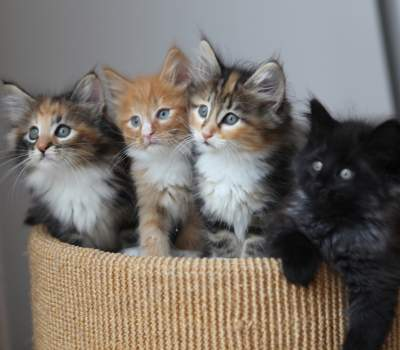
\includegraphics[width=4.16667in,height=4.16667in]{mini/images/kitten-400-350.jpeg}

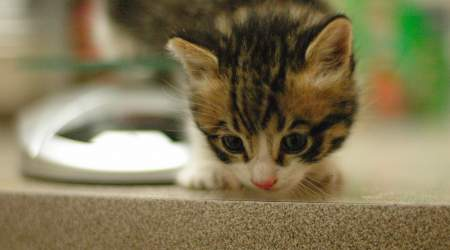
\includegraphics[width=4.6875in,height=\textheight,keepaspectratio]{mini/images/kitten-450-250.jpeg}

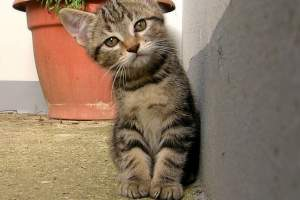
\includegraphics[width=3.125in,height=\textheight,keepaspectratio]{mini/images/kitten-300-200.jpeg}

Learn more:
\href{https://?meta:prerelease-subdomainquarto.org/docs/presentations/revealjs/advanced.html\#absolute-position}{Absolute
Position}

\subsection{Auto-Animate}\label{auto-animate}

Automatically animate matching elements across slides with Auto-Animate.

Learn more:
\href{https://?meta:prerelease-subdomainquarto.org/docs/presentations/revealjs/advanced.html\#auto-animate}{Auto-Animate}

\subsection{Auto-Animate}\label{auto-animate-1}

Automatically animate matching elements across slides with Auto-Animate.

Learn more:
\href{https://?meta:prerelease-subdomainquarto.org/docs/presentations/revealjs/advanced.html\#auto-animate}{Auto-Animate}

\subsection{Slide Transitions}\label{slide-transitions}

The next few slides will transition using the \texttt{slide} transition

\begin{longtable}[]{@{}
  >{\raggedright\arraybackslash}p{(\linewidth - 2\tabcolsep) * \real{0.1429}}
  >{\raggedright\arraybackslash}p{(\linewidth - 2\tabcolsep) * \real{0.8571}}@{}}
\toprule\noalign{}
\begin{minipage}[b]{\linewidth}\raggedright
Transition
\end{minipage} & \begin{minipage}[b]{\linewidth}\raggedright
Description
\end{minipage} \\
\midrule\noalign{}
\endhead
\bottomrule\noalign{}
\endlastfoot
\texttt{none} & No transition (default, switch instantly) \\
\texttt{fade} & Cross fade \\
\texttt{slide} & Slide horizontally \\
\texttt{convex} & Slide at a convex angle \\
\texttt{concave} & Slide at a concave angle \\
\texttt{zoom} & Scale the incoming slide so it grows in from the center
of the screen. \\
\end{longtable}

Learn more:
\href{https://?meta:prerelease-subdomainquarto.org/docs/presentations/revealjs/advanced.html\#slide-transitions}{Slide
Transitions}

\subsection{Tabsets}\label{tabsets}

\subsubsection{Plot}

\begin{Shaded}
\begin{Highlighting}[]
\FunctionTok{library}\NormalTok{(ggplot2)}
\FunctionTok{ggplot}\NormalTok{(mtcars, }\FunctionTok{aes}\NormalTok{(hp, mpg, }\AttributeTok{color =}\NormalTok{ am)) }\SpecialCharTok{+}
  \FunctionTok{geom\_point}\NormalTok{() }\SpecialCharTok{+}
  \FunctionTok{geom\_smooth}\NormalTok{(}\AttributeTok{formula =}\NormalTok{ y }\SpecialCharTok{\textasciitilde{}}\NormalTok{ x, }\AttributeTok{method =} \StringTok{"loess"}\NormalTok{)}
\end{Highlighting}
\end{Shaded}

\begin{verbatim}
Warning: The following aesthetics were dropped during statistical transformation:
colour.
i This can happen when ggplot fails to infer the correct grouping structure in
  the data.
i Did you forget to specify a `group` aesthetic or to convert a numerical
  variable into a factor?
\end{verbatim}

\pandocbounded{\includegraphics[keepaspectratio]{index_files/figure-pdf/unnamed-chunk-3-1.pdf}}

\subsubsection{Data}

\begin{Shaded}
\begin{Highlighting}[]
\NormalTok{knitr}\SpecialCharTok{::}\FunctionTok{kable}\NormalTok{(mtcars)}
\end{Highlighting}
\end{Shaded}

\begin{longtable}[]{@{}
  >{\raggedright\arraybackslash}p{(\linewidth - 22\tabcolsep) * \real{0.2778}}
  >{\raggedleft\arraybackslash}p{(\linewidth - 22\tabcolsep) * \real{0.0694}}
  >{\raggedleft\arraybackslash}p{(\linewidth - 22\tabcolsep) * \real{0.0556}}
  >{\raggedleft\arraybackslash}p{(\linewidth - 22\tabcolsep) * \real{0.0833}}
  >{\raggedleft\arraybackslash}p{(\linewidth - 22\tabcolsep) * \real{0.0556}}
  >{\raggedleft\arraybackslash}p{(\linewidth - 22\tabcolsep) * \real{0.0694}}
  >{\raggedleft\arraybackslash}p{(\linewidth - 22\tabcolsep) * \real{0.0833}}
  >{\raggedleft\arraybackslash}p{(\linewidth - 22\tabcolsep) * \real{0.0833}}
  >{\raggedleft\arraybackslash}p{(\linewidth - 22\tabcolsep) * \real{0.0417}}
  >{\raggedleft\arraybackslash}p{(\linewidth - 22\tabcolsep) * \real{0.0417}}
  >{\raggedleft\arraybackslash}p{(\linewidth - 22\tabcolsep) * \real{0.0694}}
  >{\raggedleft\arraybackslash}p{(\linewidth - 22\tabcolsep) * \real{0.0694}}@{}}
\toprule\noalign{}
\begin{minipage}[b]{\linewidth}\raggedright
\end{minipage} & \begin{minipage}[b]{\linewidth}\raggedleft
mpg
\end{minipage} & \begin{minipage}[b]{\linewidth}\raggedleft
cyl
\end{minipage} & \begin{minipage}[b]{\linewidth}\raggedleft
disp
\end{minipage} & \begin{minipage}[b]{\linewidth}\raggedleft
hp
\end{minipage} & \begin{minipage}[b]{\linewidth}\raggedleft
drat
\end{minipage} & \begin{minipage}[b]{\linewidth}\raggedleft
wt
\end{minipage} & \begin{minipage}[b]{\linewidth}\raggedleft
qsec
\end{minipage} & \begin{minipage}[b]{\linewidth}\raggedleft
vs
\end{minipage} & \begin{minipage}[b]{\linewidth}\raggedleft
am
\end{minipage} & \begin{minipage}[b]{\linewidth}\raggedleft
gear
\end{minipage} & \begin{minipage}[b]{\linewidth}\raggedleft
carb
\end{minipage} \\
\midrule\noalign{}
\endhead
\bottomrule\noalign{}
\endlastfoot
Mazda RX4 & 21.0 & 6 & 160.0 & 110 & 3.90 & 2.620 & 16.46 & 0 & 1 & 4 &
4 \\
Mazda RX4 Wag & 21.0 & 6 & 160.0 & 110 & 3.90 & 2.875 & 17.02 & 0 & 1 &
4 & 4 \\
Datsun 710 & 22.8 & 4 & 108.0 & 93 & 3.85 & 2.320 & 18.61 & 1 & 1 & 4 &
1 \\
Hornet 4 Drive & 21.4 & 6 & 258.0 & 110 & 3.08 & 3.215 & 19.44 & 1 & 0 &
3 & 1 \\
Hornet Sportabout & 18.7 & 8 & 360.0 & 175 & 3.15 & 3.440 & 17.02 & 0 &
0 & 3 & 2 \\
Valiant & 18.1 & 6 & 225.0 & 105 & 2.76 & 3.460 & 20.22 & 1 & 0 & 3 &
1 \\
Duster 360 & 14.3 & 8 & 360.0 & 245 & 3.21 & 3.570 & 15.84 & 0 & 0 & 3 &
4 \\
Merc 240D & 24.4 & 4 & 146.7 & 62 & 3.69 & 3.190 & 20.00 & 1 & 0 & 4 &
2 \\
Merc 230 & 22.8 & 4 & 140.8 & 95 & 3.92 & 3.150 & 22.90 & 1 & 0 & 4 &
2 \\
Merc 280 & 19.2 & 6 & 167.6 & 123 & 3.92 & 3.440 & 18.30 & 1 & 0 & 4 &
4 \\
Merc 280C & 17.8 & 6 & 167.6 & 123 & 3.92 & 3.440 & 18.90 & 1 & 0 & 4 &
4 \\
Merc 450SE & 16.4 & 8 & 275.8 & 180 & 3.07 & 4.070 & 17.40 & 0 & 0 & 3 &
3 \\
Merc 450SL & 17.3 & 8 & 275.8 & 180 & 3.07 & 3.730 & 17.60 & 0 & 0 & 3 &
3 \\
Merc 450SLC & 15.2 & 8 & 275.8 & 180 & 3.07 & 3.780 & 18.00 & 0 & 0 & 3
& 3 \\
Cadillac Fleetwood & 10.4 & 8 & 472.0 & 205 & 2.93 & 5.250 & 17.98 & 0 &
0 & 3 & 4 \\
Lincoln Continental & 10.4 & 8 & 460.0 & 215 & 3.00 & 5.424 & 17.82 & 0
& 0 & 3 & 4 \\
Chrysler Imperial & 14.7 & 8 & 440.0 & 230 & 3.23 & 5.345 & 17.42 & 0 &
0 & 3 & 4 \\
Fiat 128 & 32.4 & 4 & 78.7 & 66 & 4.08 & 2.200 & 19.47 & 1 & 1 & 4 &
1 \\
Honda Civic & 30.4 & 4 & 75.7 & 52 & 4.93 & 1.615 & 18.52 & 1 & 1 & 4 &
2 \\
Toyota Corolla & 33.9 & 4 & 71.1 & 65 & 4.22 & 1.835 & 19.90 & 1 & 1 & 4
& 1 \\
Toyota Corona & 21.5 & 4 & 120.1 & 97 & 3.70 & 2.465 & 20.01 & 1 & 0 & 3
& 1 \\
Dodge Challenger & 15.5 & 8 & 318.0 & 150 & 2.76 & 3.520 & 16.87 & 0 & 0
& 3 & 2 \\
AMC Javelin & 15.2 & 8 & 304.0 & 150 & 3.15 & 3.435 & 17.30 & 0 & 0 & 3
& 2 \\
Camaro Z28 & 13.3 & 8 & 350.0 & 245 & 3.73 & 3.840 & 15.41 & 0 & 0 & 3 &
4 \\
Pontiac Firebird & 19.2 & 8 & 400.0 & 175 & 3.08 & 3.845 & 17.05 & 0 & 0
& 3 & 2 \\
Fiat X1-9 & 27.3 & 4 & 79.0 & 66 & 4.08 & 1.935 & 18.90 & 1 & 1 & 4 &
1 \\
Porsche 914-2 & 26.0 & 4 & 120.3 & 91 & 4.43 & 2.140 & 16.70 & 0 & 1 & 5
& 2 \\
Lotus Europa & 30.4 & 4 & 95.1 & 113 & 3.77 & 1.513 & 16.90 & 1 & 1 & 5
& 2 \\
Ford Pantera L & 15.8 & 8 & 351.0 & 264 & 4.22 & 3.170 & 14.50 & 0 & 1 &
5 & 4 \\
Ferrari Dino & 19.7 & 6 & 145.0 & 175 & 3.62 & 2.770 & 15.50 & 0 & 1 & 5
& 6 \\
Maserati Bora & 15.0 & 8 & 301.0 & 335 & 3.54 & 3.570 & 14.60 & 0 & 1 &
5 & 8 \\
Volvo 142E & 21.4 & 4 & 121.0 & 109 & 4.11 & 2.780 & 18.60 & 1 & 1 & 4 &
2 \\
\end{longtable}

Learn more:
\href{https://?meta:prerelease-subdomainquarto.org/docs/presentations/revealjs/\#tabsets}{Tabsets}

\subsection{Interactive Slides}\label{interactive-slides}

Include Jupyter widgets and htmlwidgets in your presentations

Learn more:
\href{https://?meta:prerelease-subdomainquarto.org/docs/interactive/widgets/jupyter.html}{Jupyter
widgets},
\href{https://?meta:prerelease-subdomainquarto.org/docs/interactive/widgets/htmlwidgets.html}{htmlwidgets}

\subsection{Interactive Slides}\label{interactive-slides-1}

Turn presentations into applications with Observable and Shiny. Use
component layout to position inputs and outputs.

\begin{Shaded}
\begin{Highlighting}[]
\FunctionTok{ojs\_define}\NormalTok{(}\AttributeTok{actors =} \FunctionTok{data.frame}\NormalTok{(}
  \AttributeTok{x =} \FunctionTok{rnorm}\NormalTok{(}\DecValTok{100}\NormalTok{),}
  \AttributeTok{y =} \FunctionTok{rnorm}\NormalTok{(}\DecValTok{100}\NormalTok{)}
\NormalTok{))}
\end{Highlighting}
\end{Shaded}

\begin{Shaded}
\begin{Highlighting}[]
\NormalTok{//| panel: sidebar}
\NormalTok{viewof talentWeight = Inputs.range([{-}2, 2], \{ value: 0.7, step: 0.01, label: "talent weight" \})}
\NormalTok{viewof looksWeight = Inputs.range([{-}2, 2], \{ value: 0.7, step: 0.01, label: "looks weight" \})}
\NormalTok{viewof minimum = Inputs.range([{-}2, 2], \{ value: 1, step: 0.01, label: "min fame" \})}
\end{Highlighting}
\end{Shaded}

\begin{Shaded}
\begin{Highlighting}[]
\NormalTok{//| panel: fill}
\NormalTok{import \{ plotActors \} from \textquotesingle{}./actors.js\textquotesingle{};}
\NormalTok{plotActors(actors, talentWeight, looksWeight, minimum)}
\end{Highlighting}
\end{Shaded}

Learn more:
\href{https://?meta:prerelease-subdomainquarto.org/docs/interactive/ojs/}{Observable},
\href{https://?meta:prerelease-subdomainquarto.org/docs/interactive/shiny/}{Shiny},
\href{https://?meta:prerelease-subdomainquarto.org/docs/interactive/layout.html}{Component
Layout}

\subsection{Preview Links}\label{preview-links}

Navigate to hyperlinks without disrupting the flow of your presentation.

Use the \texttt{preview-links} option to open links in an iframe on top
of your slides. Try clicking the link below for a demonstration:

\href{https://matplotlib.org/}{Matplotlib: Visualization with Python}

Learn more:
\href{https://?meta:prerelease-subdomainquarto.org/docs/presentations/revealjs/presenting.html\#preview-links}{Preview
Links}

\subsection{Themes}\label{themes}

10 Built-in Themes (or
\href{https://?meta:prerelease-subdomainquarto.org/docs/presentations/revealjs/themes.html\#creating-themes}{create
your own})

\begin{figure}

\begin{minipage}{0.50\linewidth}
\pandocbounded{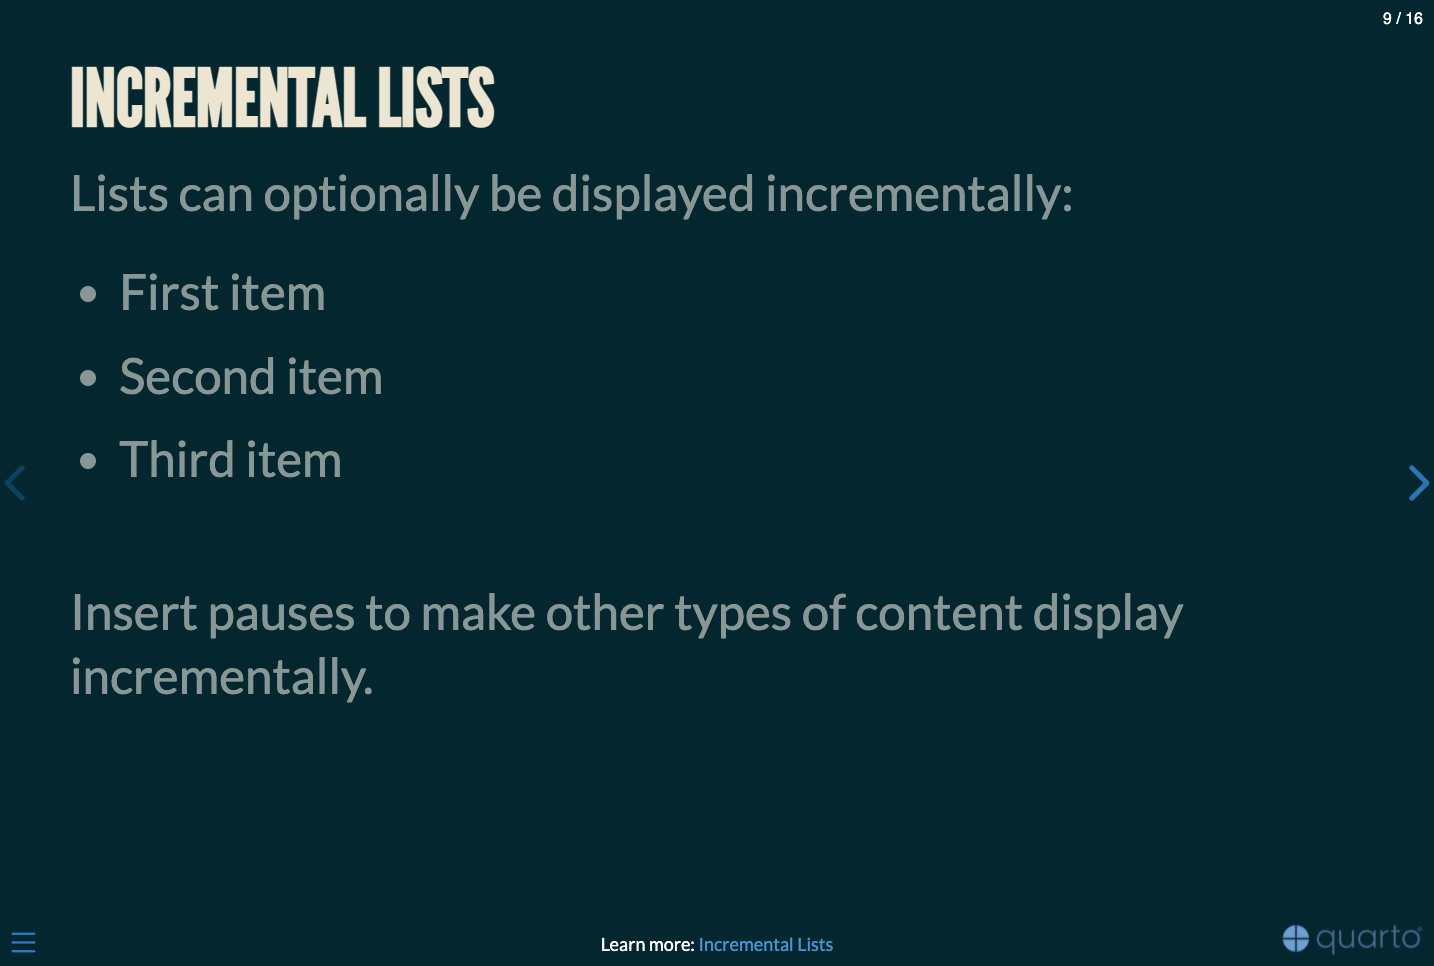
\includegraphics[keepaspectratio]{images/moon.png}}\end{minipage}%
%
\begin{minipage}{0.50\linewidth}
\pandocbounded{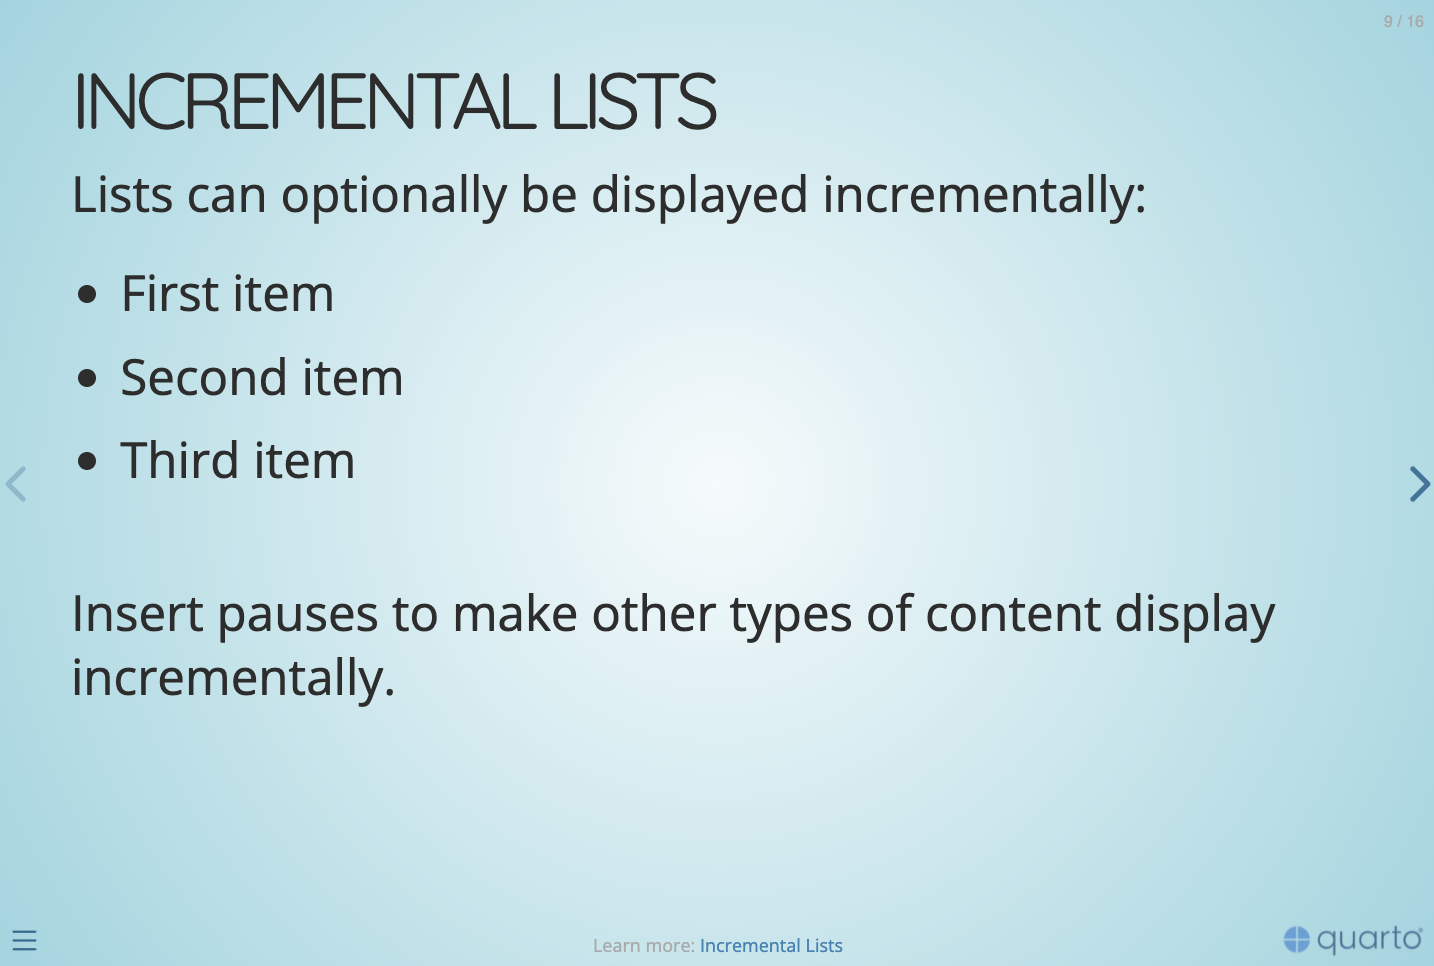
\includegraphics[keepaspectratio]{images/sky.png}}\end{minipage}%

\end{figure}%

Learn more:
\href{https://?meta:prerelease-subdomainquarto.org/docs/presentations/revealjs/themes.html}{Themes}

\subsection{Easy Navigation}\label{easy-navigation}

Quickly jump to other parts of your presentation

\begin{figure}

\begin{minipage}{0.05\linewidth}

\includegraphics[width=0.42708in,height=\textheight,keepaspectratio]{images/presentation-menu.png}\end{minipage}%
%
\begin{minipage}{0.95\linewidth}
Toggle the slide menu with the menu button (bottom left of slide) to go
to other slides and access presentation tools.\end{minipage}%

\end{figure}%

You can also press \texttt{m} to toggle the menu open and closed.

You can also press \texttt{g} to toggle `Jump To Slide' modal box to
quickly go to one of your slide using its number or id.

Learn more:
\href{./docs/presentations/revealjs/presenting.qmd\#navigation-menu}{Navigation}
/
\href{./docs/presentations/revealjs/presenting.qmd\#jump-to-slide}{Jump
To Slide}

\subsection{Jump To Slide}\label{jump-to-slide}

Quickly jump to other parts of your presentation

\subsection{Chalkboard}\label{chalkboard}

Free form drawing and slide annotations

\begin{figure}

\begin{minipage}{0.05\linewidth}

\includegraphics[width=0.42708in,height=\textheight,keepaspectratio]{images/presentation-chalkboard.png}\end{minipage}%
%
\begin{minipage}{0.95\linewidth}
Use the chalkboard button at the bottom left of the slide to toggle the
chalkboard.\end{minipage}%

\end{figure}%

\begin{figure}

\begin{minipage}{0.05\linewidth}

\includegraphics[width=0.42708in,height=\textheight,keepaspectratio]{images/presentation-notes-canvas.png}\end{minipage}%
%
\begin{minipage}{0.95\linewidth}
Use the notes canvas button at the bottom left of the slide to toggle
drawing on top of the current slide.\end{minipage}%

\end{figure}%

You can also press \texttt{b} to toggle the chalkboard or \texttt{c} to
toggle the notes canvas.

Learn more:
\href{https://?meta:prerelease-subdomainquarto.org/docs/presentations/revealjs/presenting.html\#chalkboard}{Chalkboard}

\subsection{Point of View}\label{point-of-view}

press \texttt{o} to toggle overview mode:

\pandocbounded{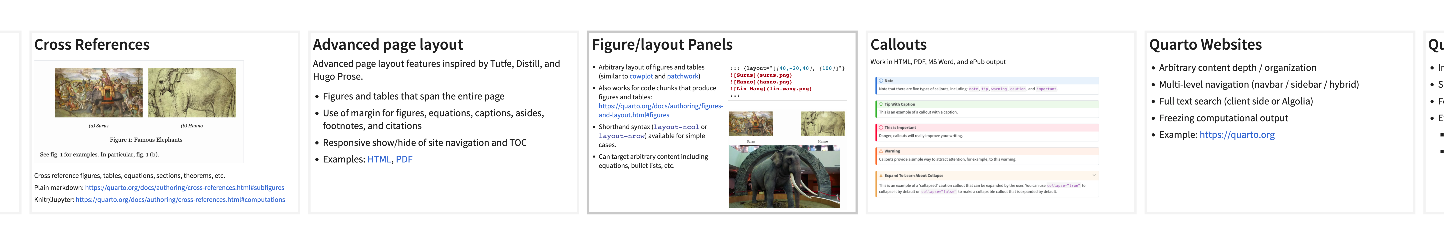
\includegraphics[keepaspectratio]{images/overview-mode.png}}

Hold down the \texttt{Alt} (linux: \texttt{Ctrl}) and click on any
element to zoom towards it---try it now on this slide.

Learn more:
\href{https://?meta:prerelease-subdomainquarto.org/docs/presentations/revealjs/presenting.html\#overview-mode}{Overview
Mode},
\href{https://?meta:prerelease-subdomainquarto.org/docs/presentations/revealjs/presenting.html\#slide-zoom}{Slide
Zoom}

\subsection{Speaker View}\label{speaker-view}

press \texttt{s} (or use the tools in presentation menu

\includegraphics[width=0.5em,height=0.5em]{../images/navigation-menu-icon.png})
to open speaker view

\begin{center}

\includegraphics[width=8.125in,height=\textheight,keepaspectratio]{images/speaker-view.png}
\end{center}

Learn more:
\href{https://?meta:prerelease-subdomainquarto.org/docs/presentations/revealjs/presenting.html\#speaker-view}{Speaker
View}

\subsection{Scroll View}\label{scroll-view}

Press \texttt{r} (or use the tools in presentation menu

\includegraphics[width=0.5em,height=0.5em]{../images/navigation-menu-icon.png})
to open scroll view

Try it now on this slide --- You'll see a scroll bar on the right and
you can scroll down the presentation using your mouse.

Scroll view behavior can be configured using \texttt{scroll-view}
configuration.

Learn more:
\href{https://?meta:prerelease-subdomainquarto.org/docs/presentations/revealjs/presenting.html\#scroll-view}{Scroll
View}

\subsection{Authoring Tools}\label{authoring-tools}

Live side-by-side preview for any notebook or text editor including
Jupyter and VS Code

\pandocbounded{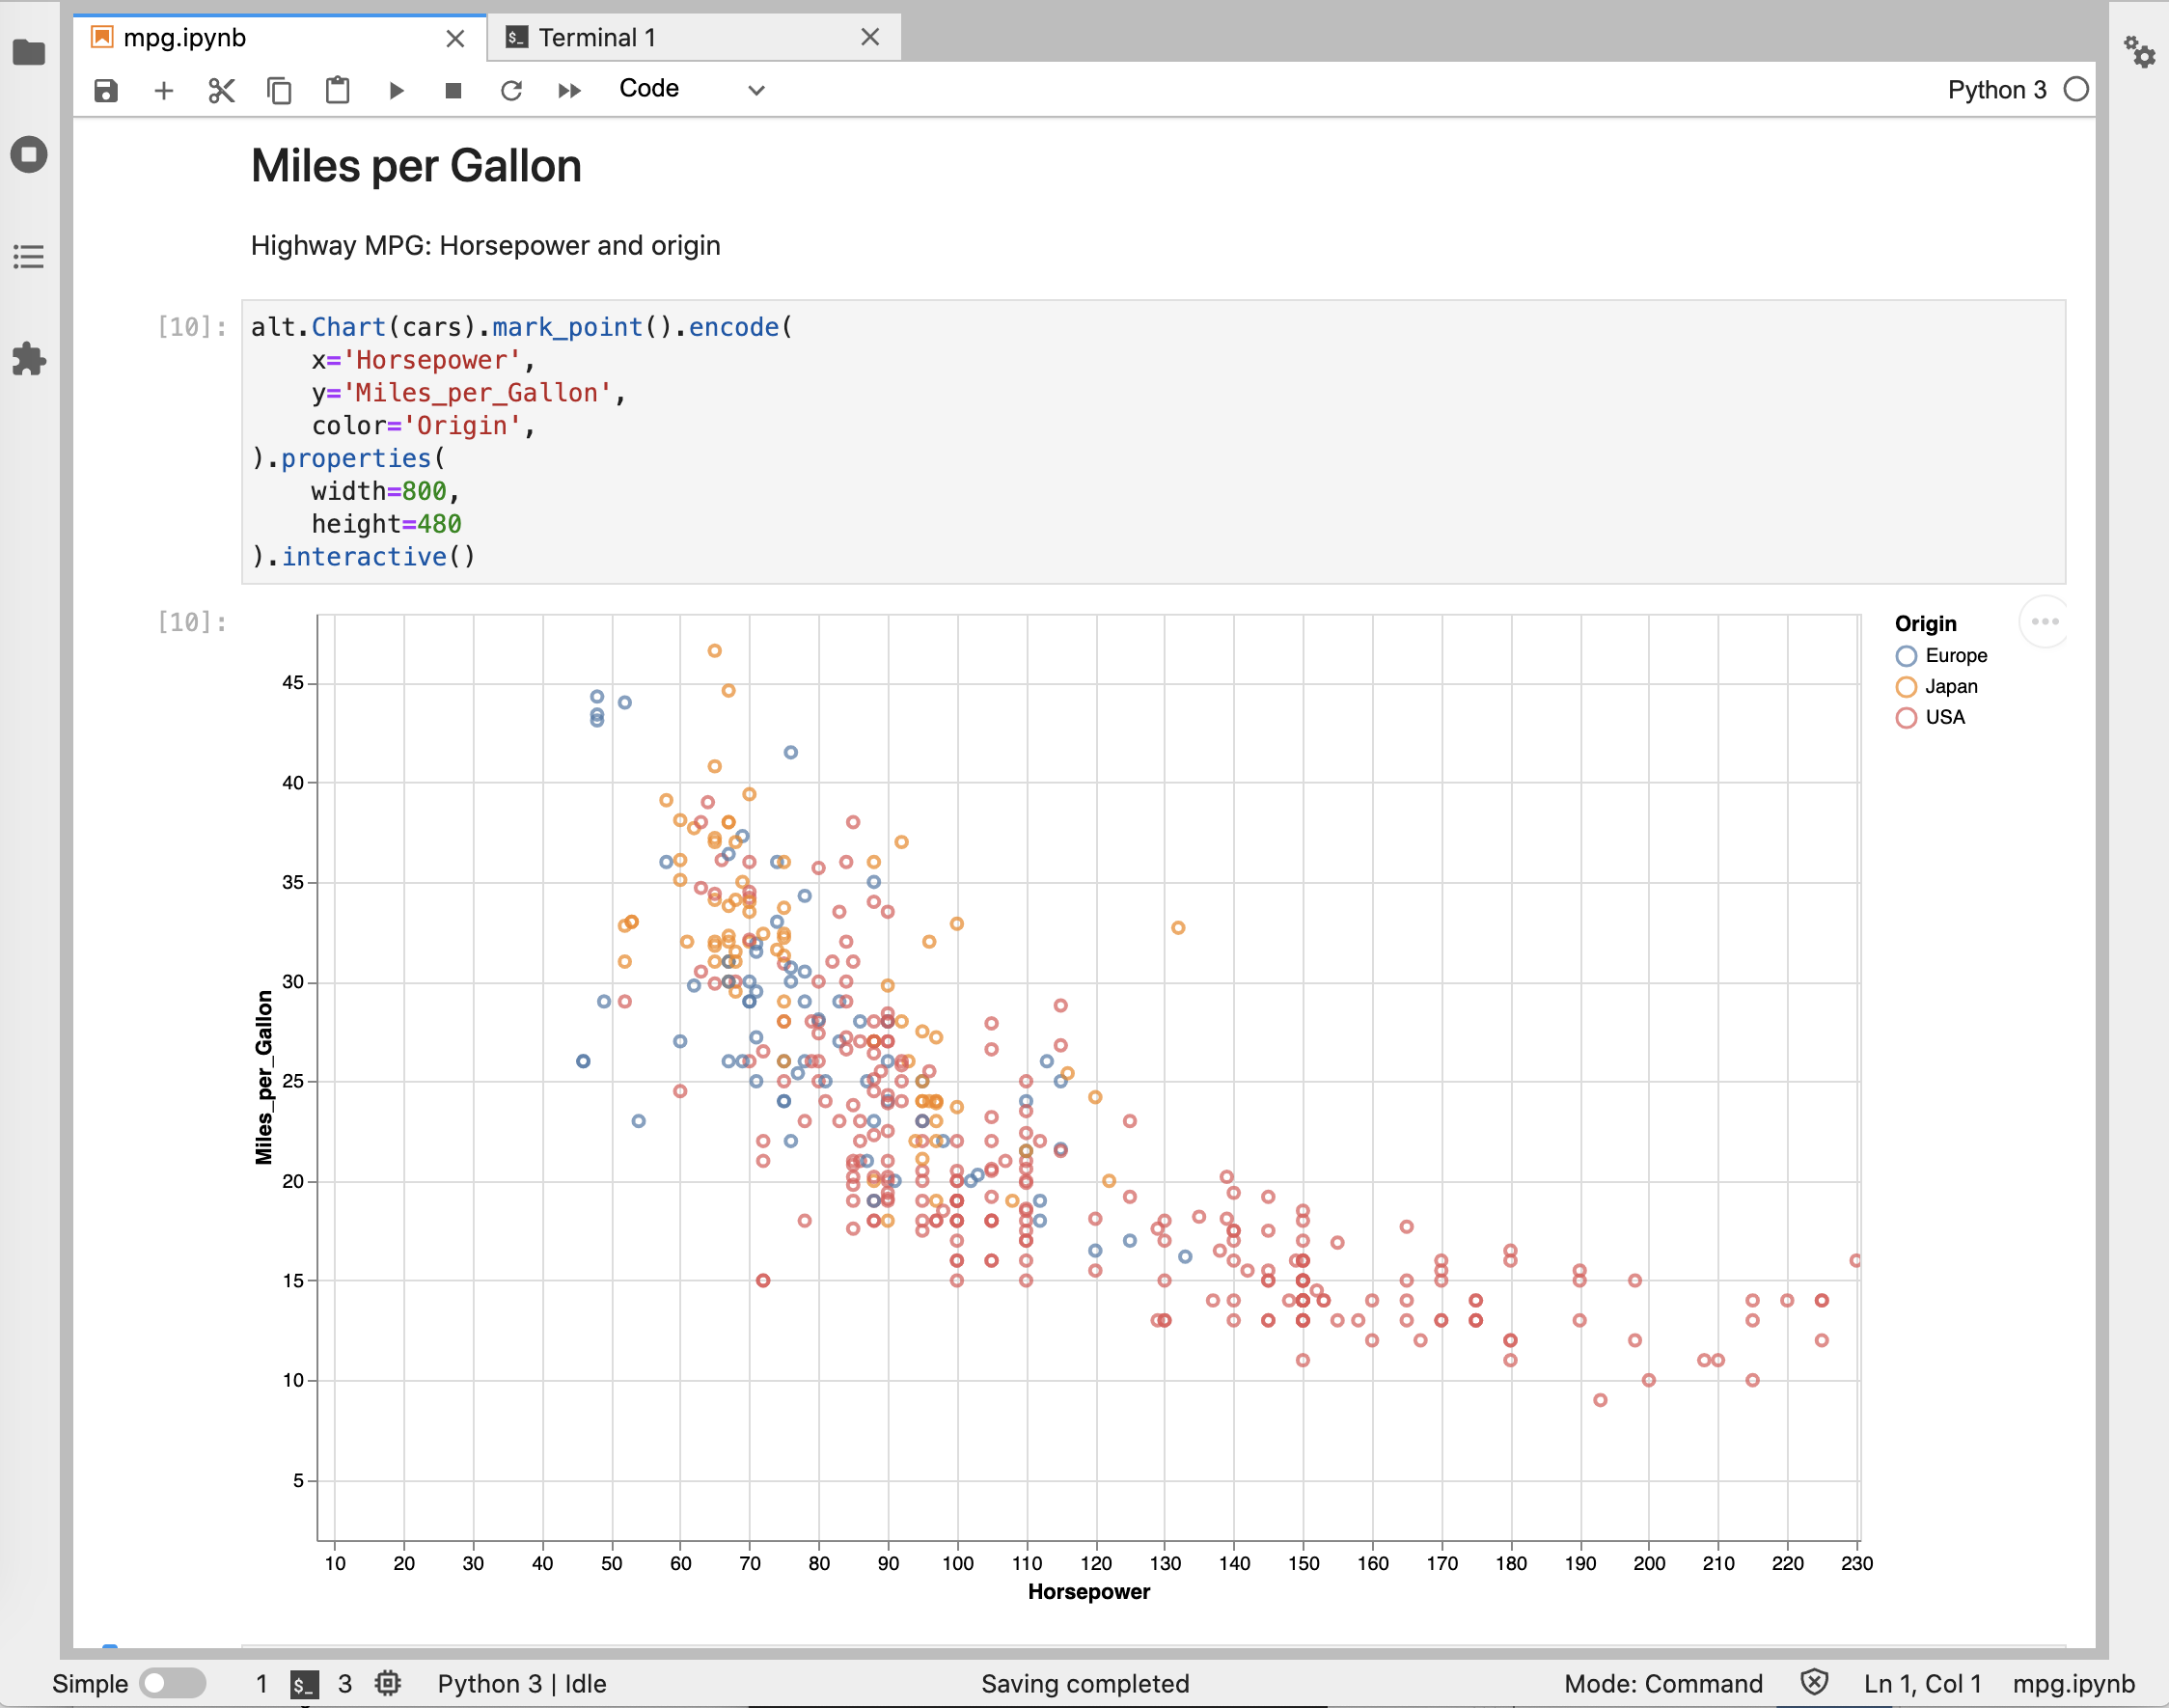
\includegraphics[keepaspectratio]{images/jupyter-edit.png}}

\pandocbounded{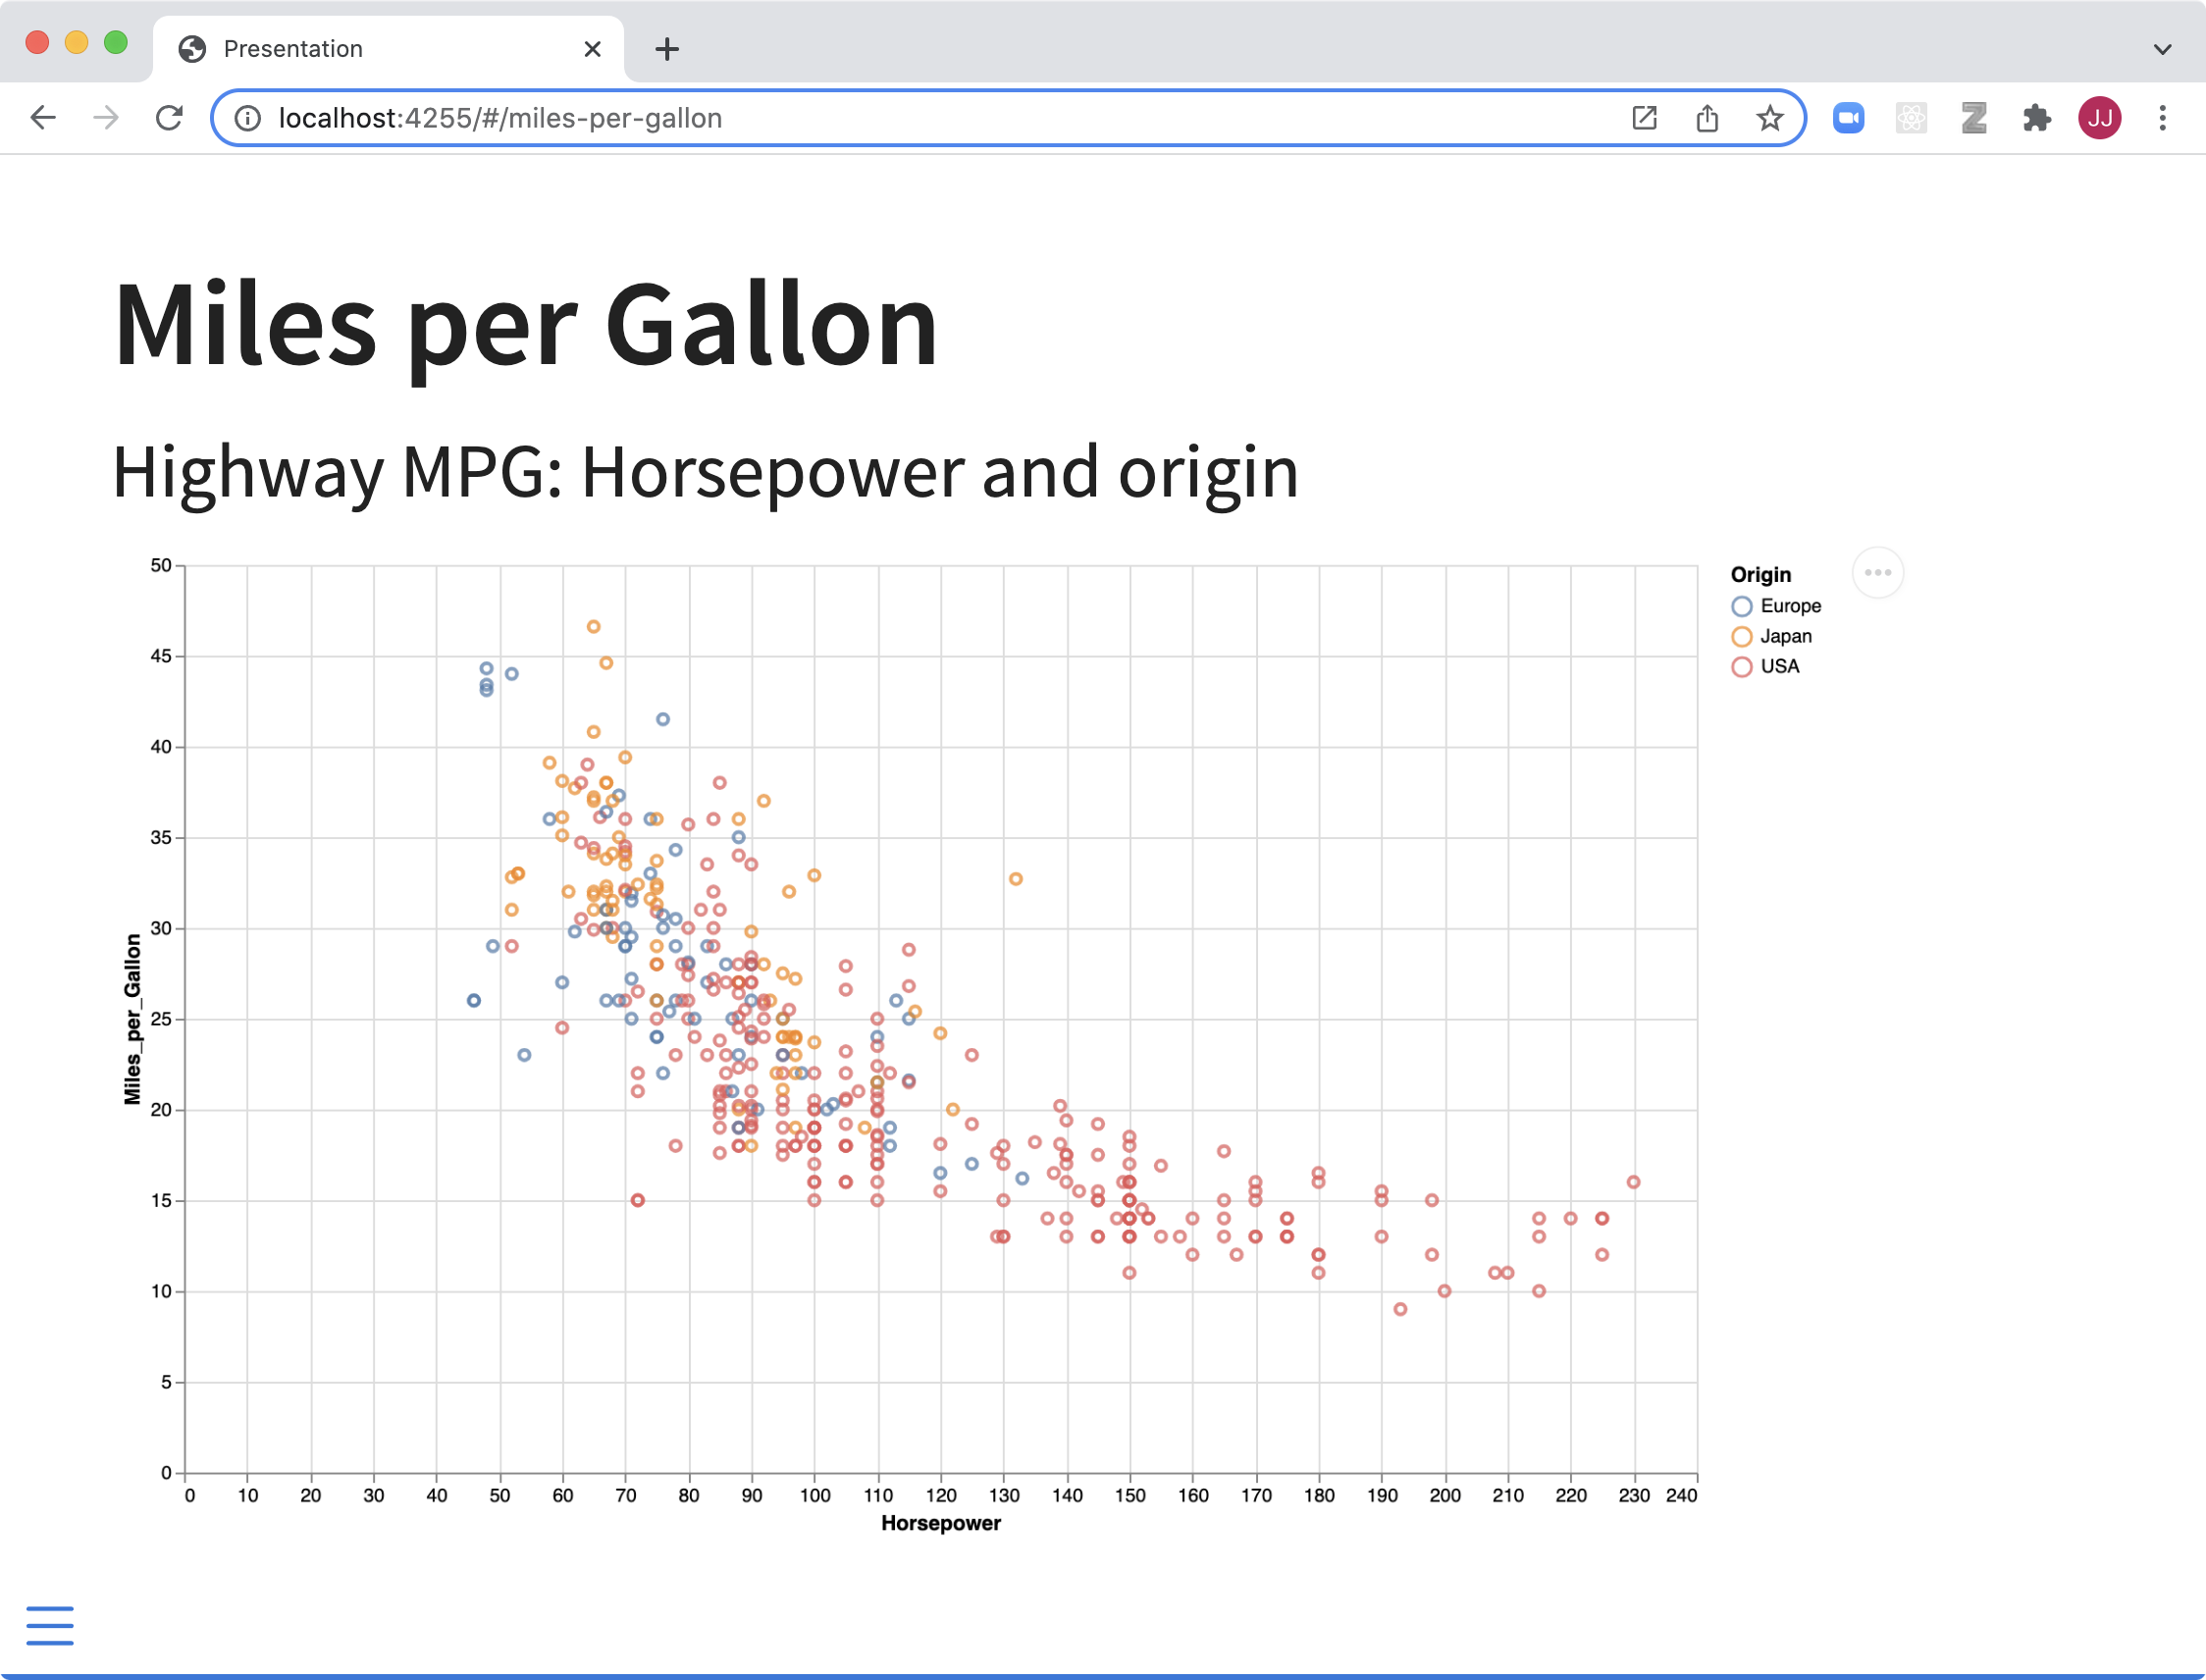
\includegraphics[keepaspectratio]{images/jupyter-preview.png}}

Learn more:
\href{https://?meta:prerelease-subdomainquarto.org/docs/tools/jupyter-lab.html}{Jupyter},
\href{https://?meta:prerelease-subdomainquarto.org/docs/tools/vscode.html}{VS
Code},
\href{https://?meta:prerelease-subdomainquarto.org/docs/tools/text-editors.html}{Text
Editors}

\subsection{Authoring Tools}\label{authoring-tools-1}

RStudio includes an integrated presentation preview pane

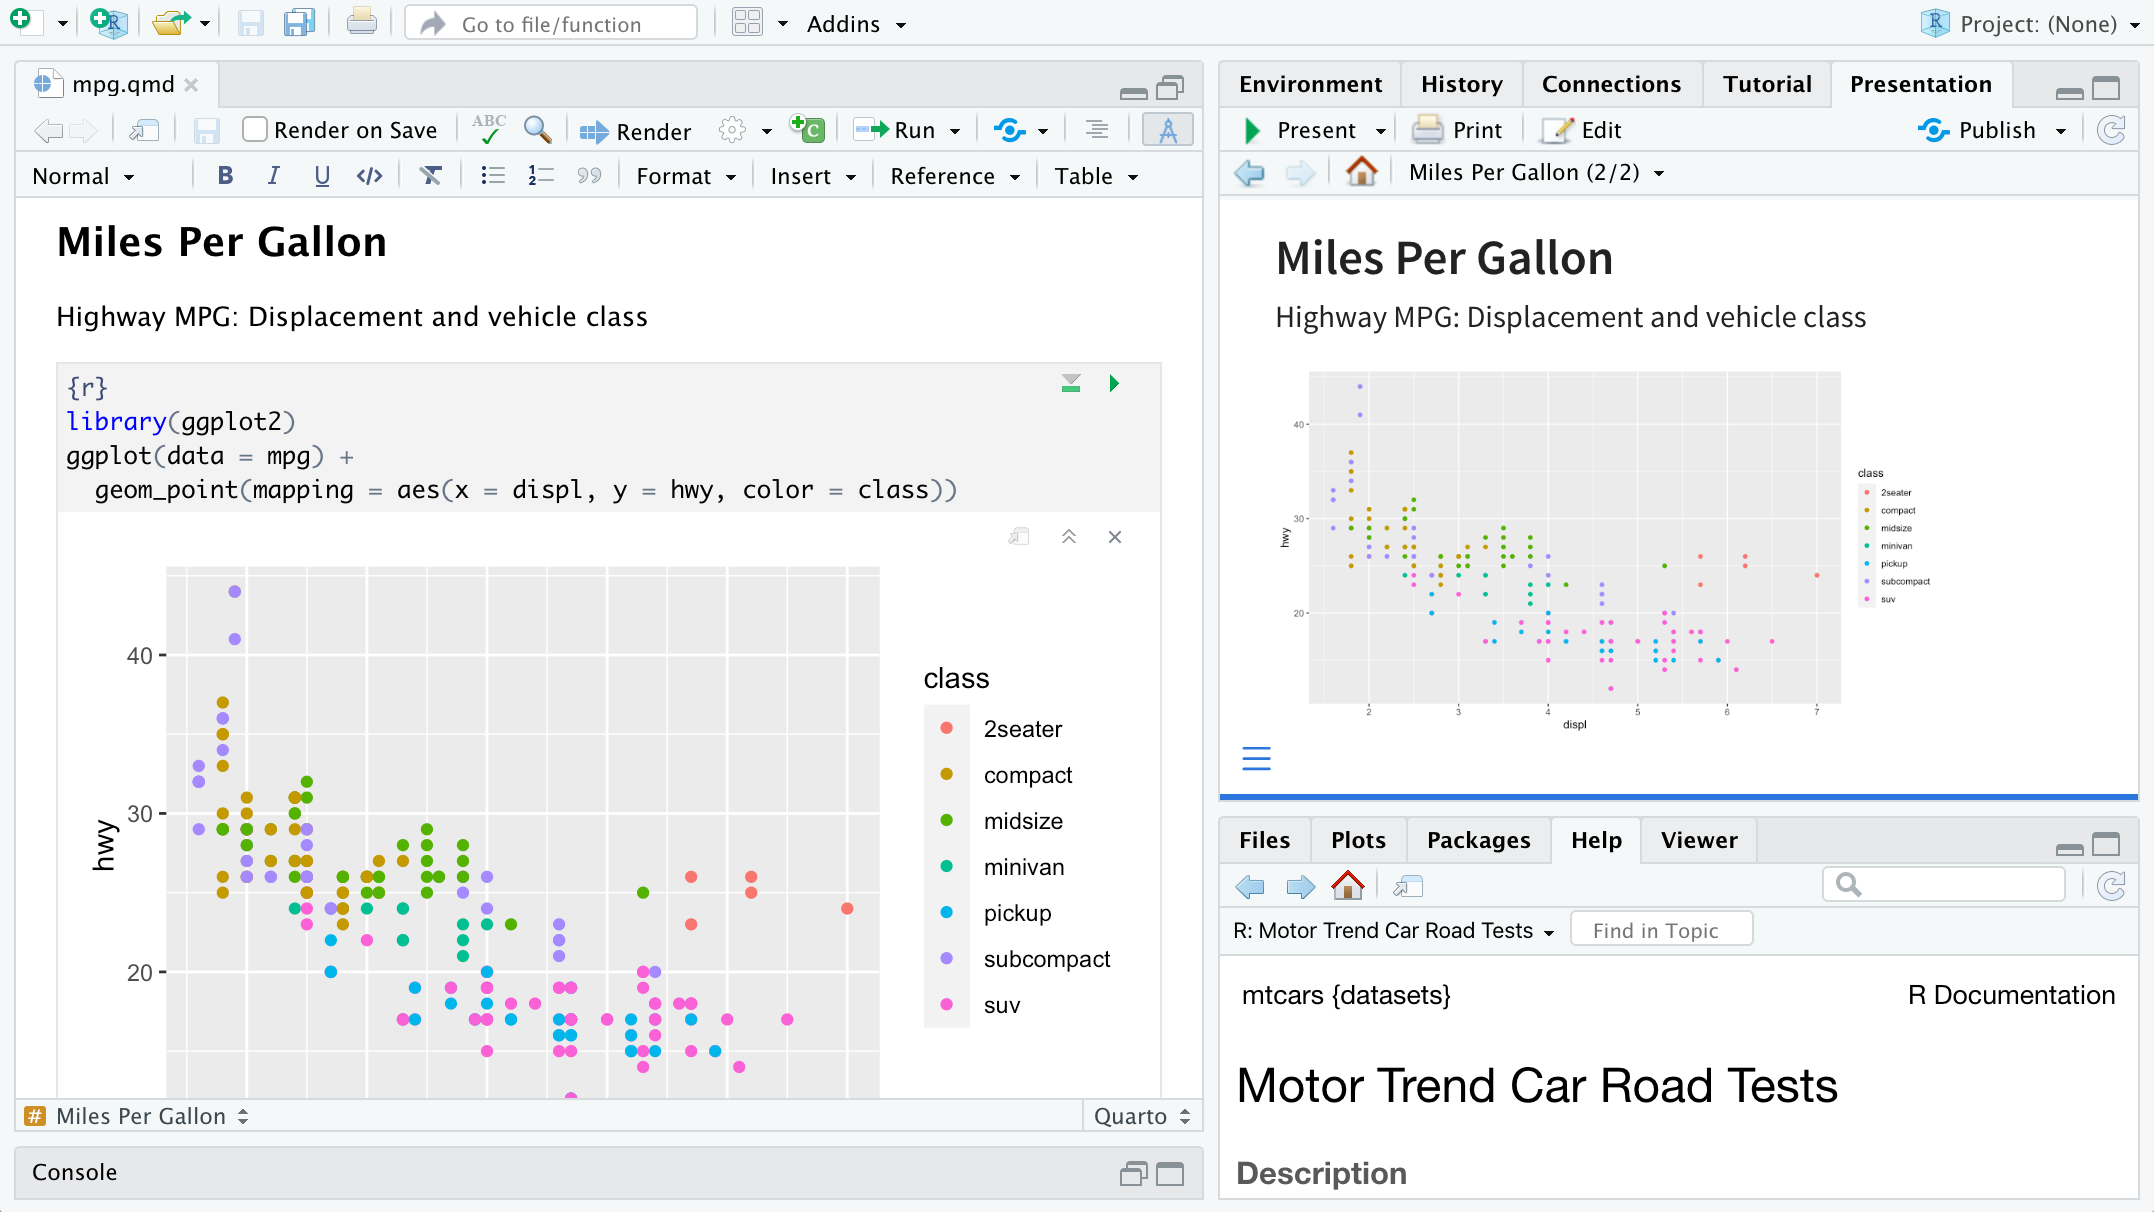
\includegraphics[width=9.375in,height=\textheight,keepaspectratio]{images/rstudio.png}

Learn more:
\href{https://?meta:prerelease-subdomainquarto.org/docs/tools/rstudio.html}{RStudio}

\subsection{And More\ldots{}}\label{and-more}

\begin{itemize}
\tightlist
\item
  \href{https://?meta:prerelease-subdomainquarto.org/docs/presentations/revealjs/advanced.html\#touch-navigation}{Touch}
  optimized (presentations look great on mobile, swipe to navigate
  slides)
\item
  \href{https://?meta:prerelease-subdomainquarto.org/docs/presentations/revealjs/\#footer-logo}{Footer
  \& Logo} (optionally specify custom footer per-slide or hide global
  footer)
\item
  \href{https://?meta:prerelease-subdomainquarto.org/docs/presentations/revealjs/presenting.html\#auto-slide}{Auto-Slide}
  (step through slides automatically, without any user input)
\item
  \href{https://?meta:prerelease-subdomainquarto.org/docs/presentations/revealjs/presenting.html\#multiplex}{Multiplex}
  (allows your audience to follow the slides of the presentation you are
  controlling on their own phone, tablet or laptop).
\end{itemize}

Learn more:
\href{https://?meta:prerelease-subdomainquarto.org/docs/presentations/revealjs/}{Quarto
Presentations}

\subsection{References}\label{references}

\phantomsection\label{refs}
\begin{CSLReferences}{1}{0}
\bibitem[\citeproctext]{ref-chishtieUseEpicElectronic2023}
Chishtie, Jawad, Natalie Sapiro, Natalie Wiebe, Leora Rabatach, Diane
Lorenzetti, Alexander A. Leung, Doreen Rabi, Hude Quan, and Cathy A.
Eastwood. 2023. {``Use of {Epic Electronic Health Record System} for
{Health Care Research}: {Scoping Review}.''} \emph{Journal of Medical
Internet Research} 25 (December): e51003.
\url{https://doi.org/10.2196/51003}.

\bibitem[\citeproctext]{ref-schadow1999units}
Schadow, Gunther, Clement J McDonald, Jeffrey G Suico, Ulrich Föhring,
and Thomas Tolxdorff. 1999. {``Units of Measure in Clinical Information
Systems.''} \emph{Journal of the American Medical Informatics
Association} 6 (2): 151--62.

\end{CSLReferences}




\end{document}
